\documentclass[11pt]{article}

\usepackage[a4paper,margin=1in]{geometry}
\usepackage{amsmath,amsfonts,amssymb}
\usepackage{graphicx}
\usepackage{booktabs,longtable}
\usepackage{pdfpages}
\usepackage[hidelinks]{hyperref}
\usepackage{xurl}
\setlength{\emergencystretch}{8em}

\title{$k=1$ ($K=2$) lazy ring + directed shortcut:\\Equal-probability baseline away from the shortcut source (stay/left/right each $1/3$)\\Bimodality via Chebyshev analytic generating function + AW inversion (flux cross-check)}
\author{}
\date{}

\begin{document}
\sloppy
\maketitle

\section{Model (simplest case: $k=1$ / $K=2$)}
We consider a ring with nodes $0,1,\dots,N-1$ and a lazy nearest-neighbor random walk:
\[
P(i\to i)=1-q,\qquad P(i\to i\pm1)=\frac{q}{2}\quad(\mathrm{mod}\ N),
\qquad 0<q<1.
\]
For the \emph{equal-probability} baseline (stay/left/right each $1/3$),
\[
1-q=\frac{q}{2}=\frac{1}{3}\quad\Longleftrightarrow\quad q=\frac{2}{3}.
\]
We add one directed shortcut $u\to v$ using the ``take probability from the self-loop'' model:
\[
P(u\to u)=1-q-p,\qquad P(u\to v)=p,\qquad 0\le p\le 1-q.
\]
Note: the phrase “equal-probability” here refers to the \emph{non-shortcut} nodes (stay/left/right each $1/3$ when $q=2/3$).
It does \emph{not} mean that the shortcut source $u$ has four equal actions; the “equal4” rule (stay/left/right/shortcut each $1/4$ at $u$)
is treated separately in Section~\ref{sec:equal4-en}.
The target node $\mathrm{target}$ is absorbing. We study the first-passage-time pmf
\[
f(t)=\Pr(T=t),\qquad t=1,2,\dots
\]
from the start node $n_0$ to $\mathrm{target}$ and ask whether $f(t)$ is bimodal.

\section{Analytic inversion (AW) and flux cross-check}
\paragraph{Does laziness change the analytic formula?}
The lazy parameter $q\in(0,1)$ enters the spectrum directly: the defect-free eigenvalues are
$\lambda_k=1-q+q\cos(2\pi k/N)$.
The full closed form (including the directed shortcut and the ``from self-loop'' construction) is given in
\texttt{deriv\_k2/note\_k2.pdf}
as a Chebyshev representation of $\tilde Q(d,z)$, $\tilde S_{n_0}(n,z)$, and $\tilde F_{n_0\to n}(z)$.

\paragraph{AW inversion}
Given $\tilde F(z)=\sum_{t\ge0} f(t)z^t$, we recover coefficients by discrete Cauchy inversion:
sample $z_k=r e^{2\pi i k/m}$ and compute
\[
f(t)\approx r^{-t}\frac{1}{m}\sum_{k=0}^{m-1}\tilde F(z_k)\,e^{-2\pi i k t/m},
\qquad t=1,2,\dots
\]
implemented via FFT. Our implementation is \texttt{lazy\_ring\_aw\_chebyshev.py}.

\paragraph{Flux recursion (validation)}
We also compute $f(t)$ by time-domain propagation with an absorbing target and record the flux into it:
\[
f(t+1)=\sum_{i\neq \mathrm{target}} p_t(i)\,P(i\to \mathrm{target}).
\]
Implementation: \texttt{lazy\_ring\_flux\_bimodality.py}.

\section{Bimodality criteria (paper-style + macro separation)}\label{sec:criterion-en}
For discrete-time nearest-neighbor walks, $f(t)$ can exhibit genuine small-$t$ micro-structure.
We therefore use strict local maxima with a threshold:
\begin{itemize}
  \item \textbf{Strict local peak:} $f(t)>f(t-1)$, $f(t)>f(t+1)$, and $f(t)\ge h_{\min}$.
  \item \textbf{Paper bimodality:} at least two peaks, and the 2nd-highest peak height $\ge 1\%$ of the highest.
  \item \textbf{Macro bimodality (optional):} additionally require $t_2/t_1\ge 10$ for the two dominant peaks.
\end{itemize}

\section{Key findings}
Under the $k=1$ ($K=2$) lazy ring with one directed shortcut, the following reproducible conclusions hold (analytic AW inversion with flux cross-check):
\begin{itemize}
  \item \textbf{Selfloop (take $p$ from the self-loop) can be bimodal for small $p$:} the minimal case
  $N=10,q=2/3,u=n_0=1\to v=\mathrm{target}=5,p=0.006666\ldots$ has exactly two strict local peaks under $h_{\min}=10^{-7}$
  (Section~\ref{sec:min-en}, Figure~\ref{fig:n10-example-en}); the odd-$N$ case $N=11$ shows the same peak pair (Figure~\ref{fig:n11-example-en}).
  \item \textbf{Full scan indicates macro-bimodality starts at $N=10$:} for $q=2/3$, $\beta=0.02$, and the shortcut $u=n_0\to v=\mathrm{target}$,
  a scan over all endpoints for $N=3..60$ finds macro-bimodality mainly at large ring distances (heatmap + Appendix table).
  \item \textbf{Equal4 (four actions each $1/4$ at $u$) is unimodal for the paper-like geometry:} scanning $N=10..200$ for the paper-like offsets
  $(u,v)=(n_0+5,\mathrm{target}+1)$ yields zero paper/macro bimodality cases (Section~\ref{sec:equal4-en}).
  \item \textbf{Large shortcut strength suppresses bimodality:} for the paper-like geometry at $N=100$ ($u=6\to v=51$),
  the $\beta$ scan shows paper/macro flags drop to 0 once $\beta\gtrsim 0.07$ (Table~\ref{tab:selfloop-beta-scan-en}, Figure~\ref{fig:selfloop-beta-sens-en}).
\end{itemize}

\section{Minimal clean example: $N=10$ (selfloop model; not equal4)}\label{sec:min-en}
Parameters:
\begin{itemize}
  \item $N=10$, $q=2/3$ (equal-prob baseline);
  \item $n_0=1$, $\mathrm{target}=5$;
  \item shortcut (selfloop rule; \textbf{not} $1/4$ each at $u$): $u=n_0=1\to v=\mathrm{target}=5$, $p=0.006666\ldots$ (e.g.\ $\beta=0.02$ so $p=\beta(1-q)=0.02/3$);
  \item flux run stops at survival $<10^{-14}$ (tail-mass upper bound).
\end{itemize}
With $h_{\min}=10^{-7}$ this case has exactly two strict local peaks, at $t_1=1$ and $t_2=10$, and satisfies $t_2/t_1=10$.
\begin{figure}[!htbp]
  \centering
  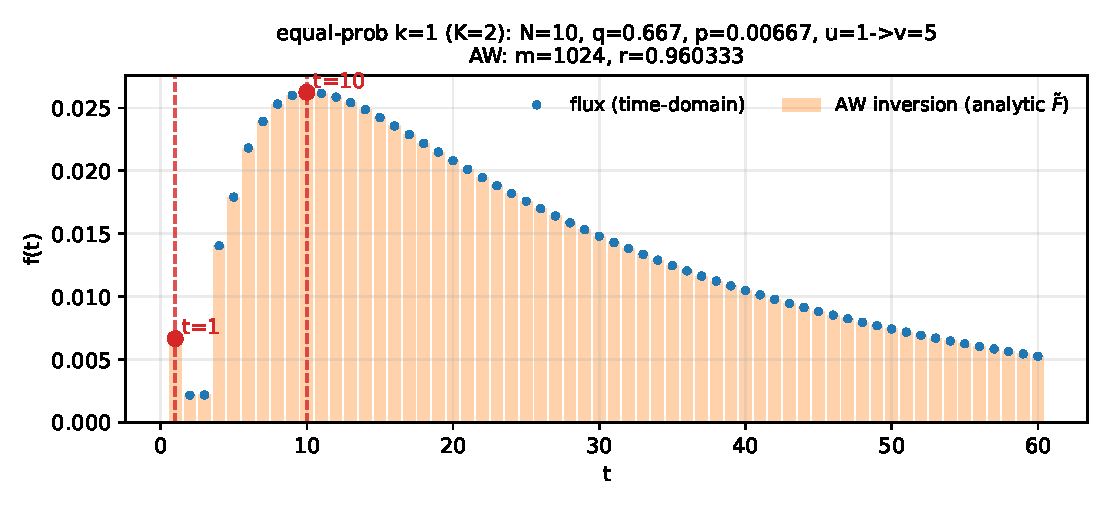
\includegraphics[width=0.92\linewidth]{figures/lazy_ring_flux_bimodality/lazy_K2_equalprob_N10_aw_vs_flux.pdf}
  \caption{$N=10,q=2/3,p=0.006666\ldots,u=1\to v=5$. AW inversion (analytic $\tilde F$) matches flux; two peak times are marked.}
  \label{fig:n10-example-en}
\end{figure}

\section{Odd $N$ example: $N=11$}
Using the same baseline and shortcut setting ($u=n_0=1\to v=\mathrm{target}=5$, $p=0.006666\ldots$), we also get two strict peaks
at $t_1=1,t_2=10$ (with $h_{\min}=10^{-7}$).
\begin{figure}[!htbp]
  \centering
  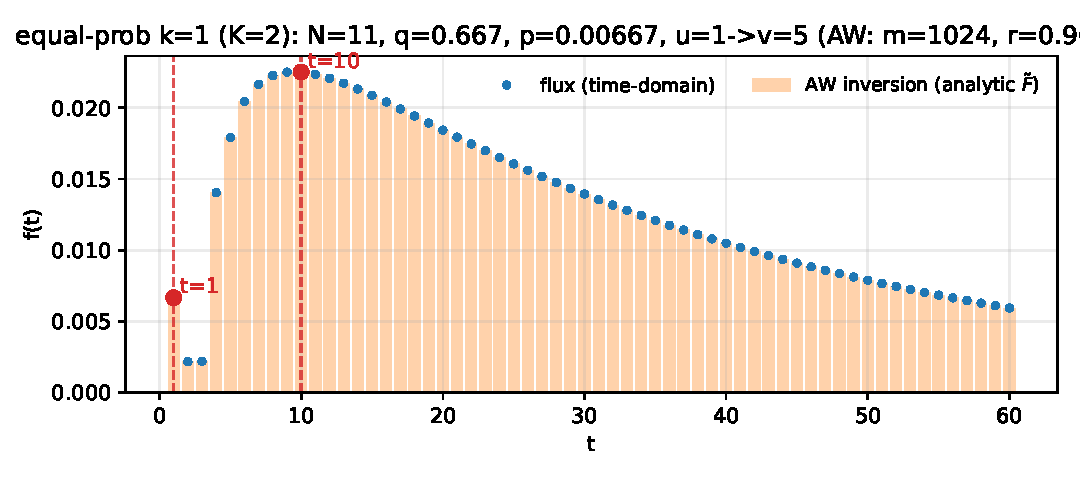
\includegraphics[width=0.92\linewidth]{figures/lazy_ring_flux_bimodality/lazy_K2_equalprob_N11_target5_aw_vs_flux.pdf}
  \caption{$N=11$ (odd) example; AW and flux overlap to machine precision.}
  \label{fig:n11-example-en}
\end{figure}

\section{Full scan (AW analytic): $N$ from small to larger}
We fix $q=2/3$, $n_0=1$, and the simplest shortcut $u=n_0\to v=\mathrm{target}$ with $\beta=0.02$ (so $p=0.006666\ldots$),
and scan all endpoints $\mathrm{target}\neq n_0$ for $N=3..60$.

\paragraph{Scan protocol}
For each $(N,\mathrm{target})$:
\begin{itemize}
  \item evaluate $\tilde F(z)$ from the Chebyshev closed form (\texttt{lazy\_ring\_aw\_chebyshev.py});
  \item invert by AW to obtain $f(t)$ up to $t_{\max}=\lceil 4N^2\rceil$;
  \item choose $m=\mathrm{pow2}(\mathrm{oversample}\cdot(t_{\max}+1))$ (default \texttt{oversample=4}) and $r$ so that $r^m=10^{-18}$;
  \item detect strict local peaks ($h_{\min}=10^{-7}$) and compute paper/macro flags and dominant peak times $(t_1,t_2)$.
\end{itemize}
The complete per-target table is in Appendix Table~\ref{tab:fullscan-en}.

\paragraph{Heatmap view}
We visualize where \emph{macro bimodality} holds ($t_2/t_1\ge 10$) and color those points by the late peak time $t_2$.
The horizontal axis is the ring distance $d=\mathrm{dist}(n_0,\mathrm{target})$ and the vertical axis is $N$.
\begin{figure}[!htbp]
  \centering
  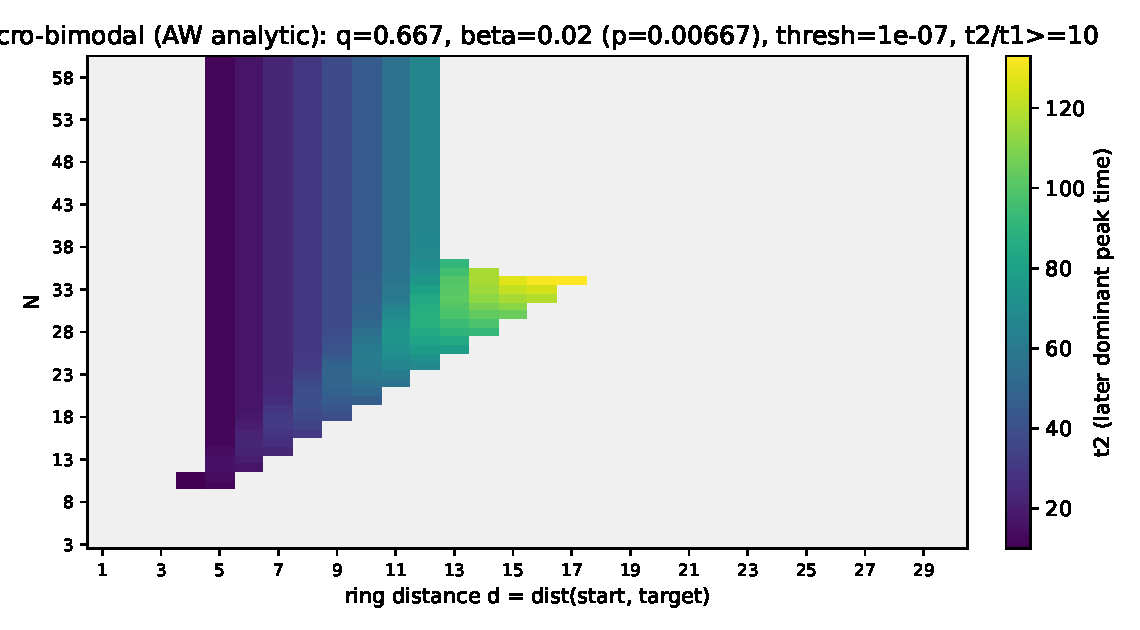
\includegraphics[width=0.92\linewidth]{figures/lazy_ring_flux_bimodality/lazy_K2_equalprob_macro_scan_N3_60.pdf}
  \caption{Full scan heatmap (AW analytic): $N=3..60$, distance $d$, and macro-bimodality locations; color shows the late peak time $t_2$.}
\end{figure}

\section{The “equal shortcut probability” rule: equal4 (four actions each $1/4$ at $u$)}\label{sec:equal4-en}
The Chebyshev closed form in \texttt{deriv\_k2/note\_k2.pdf} corresponds to the \emph{selfloop} rule:
take probability $p$ from the self-loop at $u$ and add it to $u\to v$, while keeping $P(u\to u\pm1)=q/2$ unchanged.

If the shortcut is chosen with the \emph{same probability as the other actions} at the source $u$,
then the rule at $u$ is
\[
P(u\to u)=P(u\to u\pm1)=P(u\to v)=\frac14,
\]
which also changes the neighbor probabilities at $u$ (so the closed form changes).
This is still a \textbf{single-column defect} and can be handled analytically by a rank-1 (Sherman--Morrison) update of the
defect-free propagator $\tilde Q(z)$; we implement this as \texttt{fpt\_pmf\_aw\_equal4} in \texttt{lazy\_ring\_aw\_chebyshev.py}
and cross-check it by flux.

\paragraph{Conclusion (no bimodality for the paper-like geometry)}
For the repeatedly used paper-like geometry
($n_0=1$, $\mathrm{target}=\lfloor N/2\rfloor$, $u=n_0+5$, $v=\mathrm{target}+1$),
a scan over $N=10..200$ finds \textbf{zero} paper/macro-bimodality cases under the equal4 rule
($h_{\min}=10^{-7}$, 2nd peak $\ge 1\%$, and macro separation $t_2/t_1\ge 10$).
Representative rows are listed in Table~\ref{tab:equal4-paper-geom-en}.
Figure~\ref{fig:paper-geom-equal4-compare-en} shows a direct comparison at $N=100$:
the selfloop small-$p$ model exhibits two dominant peaks, while the equal4 rule yields a single peak.
\begin{table}[!htbp]
\centering
\small
\begin{tabular}{rrrrrr}
\toprule
$N$ & $u$ & $v$ & paper & macro & $t_\mathrm{peak}$\\
\midrule
20 & 6 & 11 & 0 & 0 & 34\\
50 & 6 & 26 & 0 & 0 & 27\\
100 & 6 & 51 & 0 & 0 & 27\\
160 & 6 & 81 & 0 & 0 & 27\\
200 & 6 & 101 & 0 & 0 & 27\\
\bottomrule
\end{tabular}
\caption{Representative results under the equal-4 rule at the shortcut source (at $u$: stay/left/right/shortcut each $1/4$), using the paper-like geometry $n_0=1$, $\mathrm{target}=\lfloor N/2\rfloor$, $u=n_0+5$, $v=\mathrm{target}+1$.}
\label{tab:equal4-paper-geom-en}
\end{table}

\begin{figure}[!htbp]
  \centering
  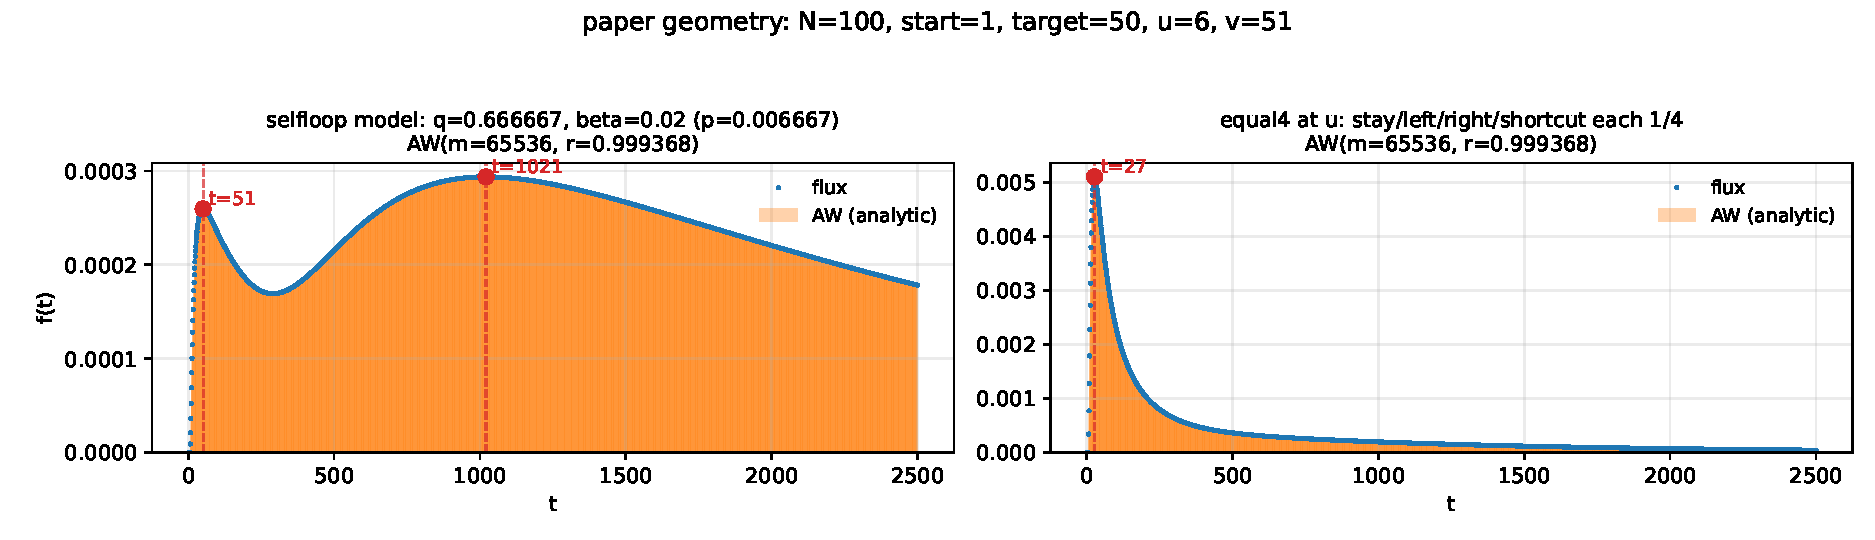
\includegraphics[width=0.98\linewidth]{figures/lazy_ring_flux_bimodality/lazy_K2_paper_geometry_selfloop_vs_equal4_N100.pdf}
  \caption{Paper-like geometry ($N=100$, $u=6\to v=51$): selfloop (left) is bimodal for $\beta=0.02$; equal4 (right) is unimodal. AW inversion matches flux in both.}
  \label{fig:paper-geom-equal4-compare-en}
\end{figure}

\subsection{Why does bimodality disappear for large $p$? (selfloop $\beta$ scan)}
Intuitively, in the selfloop construction, increasing $p$ makes it much more likely to enter the shortcut before reaching $\mathrm{target}$,
concentrating mass at a faster time scale and suppressing the slower diffusive peak.
For the paper-like geometry at $N=100$ ($u=6\to v=51$), a $\beta$ scan ($p=\beta(1-q)$) shows that for $\beta\gtrsim 0.07$
the paper/macro bimodality flags drop to 0 (Table~\ref{tab:selfloop-beta-scan-en}), and the curves become unimodal
(Figure~\ref{fig:selfloop-beta-sens-en}).

\input{tables/lazy_K2_selfloop_beta_scan_N100_en.tex}
\begin{figure}[!htbp]
  \centering
  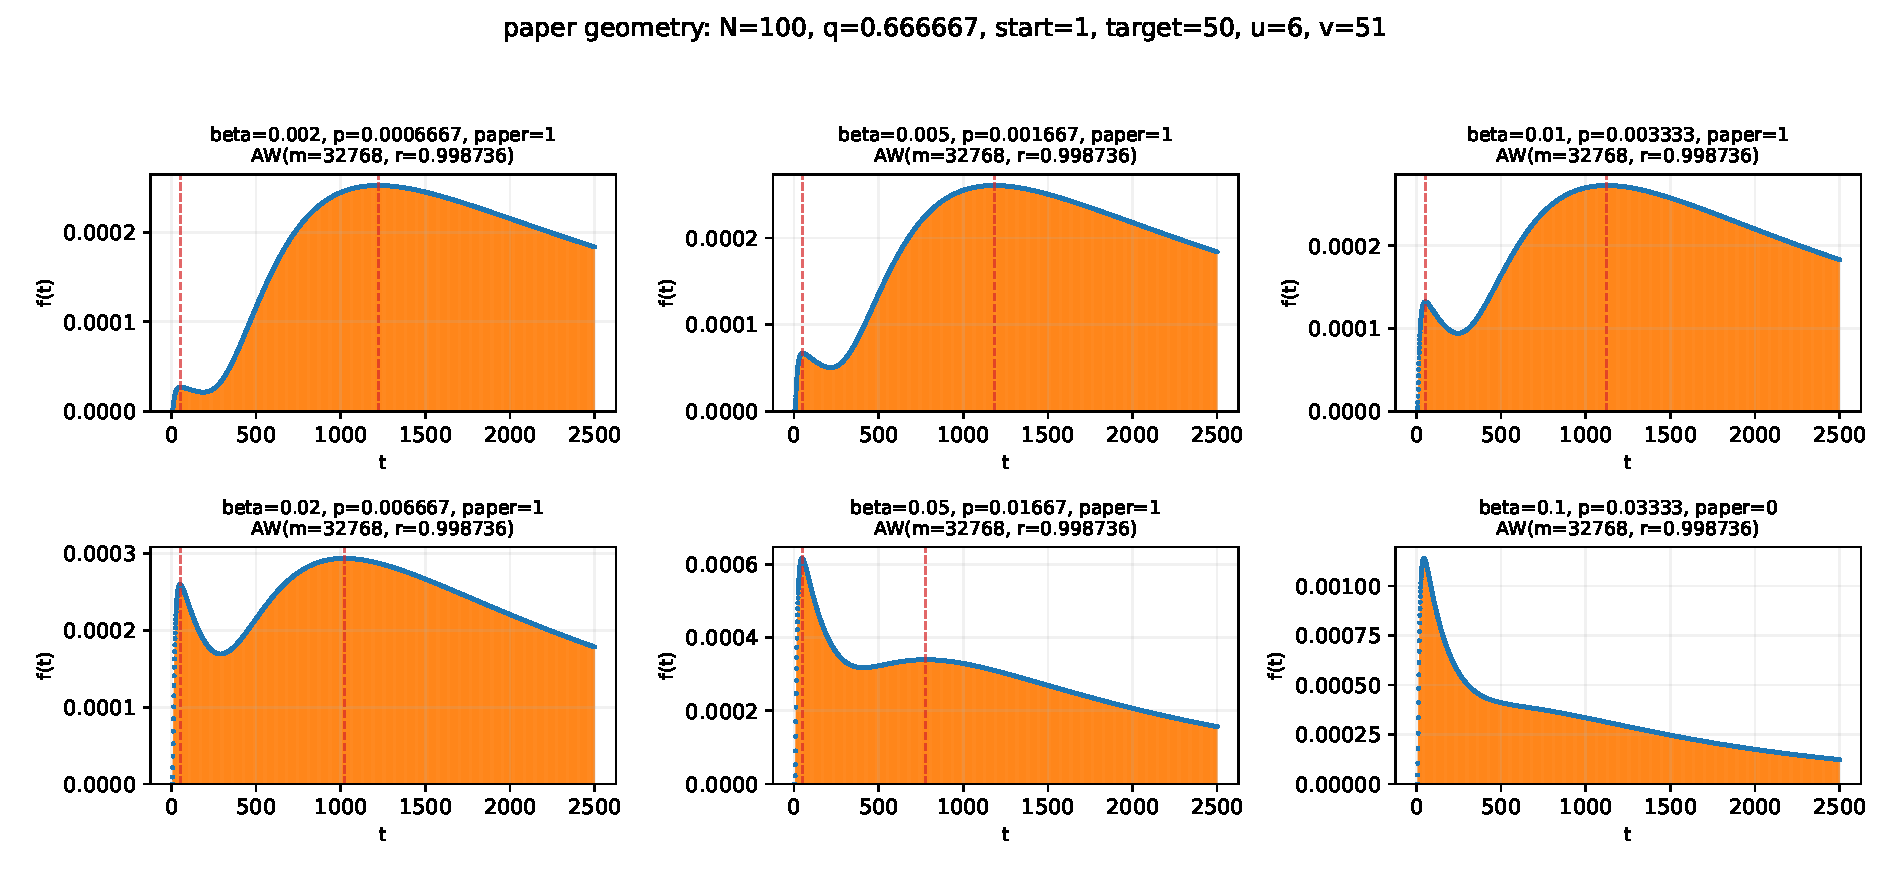
\includegraphics[width=0.98\linewidth]{figures/lazy_ring_flux_bimodality/lazy_K2_selfloop_beta_sensitivity_N100.pdf}
  \caption{Selfloop $\beta$ sensitivity at the paper-like geometry ($N=100$, $u=6\to v=51$), with $p=\beta(1-q)$. Increasing $p$ suppresses bimodality. Each panel overlays analytic AW inversion with flux.}
  \label{fig:selfloop-beta-sens-en}
\end{figure}

\section{Comparison: why does \texttt{valley\_report} show “no bimodality” for $K=2$?}
\texttt{ring\_valley.tex} / \texttt{valley\_study.py} use a different construction (closer to the original paper Fig.~3 setup):
\begin{itemize}
  \item \textbf{Non-lazy walk:} uniform jump to $K$ neighbors (no self-loop).
  \item \textbf{Shortcut probability rule:} at the shortcut source node, \emph{add} a directed edge and renormalize all outgoing probabilities to $1/(K+1)$ (each original neighbor edge drops from $1/K$ to $1/(K+1)$).
  \item \textbf{Parity fix for $K=2$:} coarse-grain by 2 steps before applying the Fig.~3 peak rule.
\end{itemize}
Under this model, the $K=2$ scan reports no bimodality over wide $N$ ranges. We reproduce that with an exact master-equation propagation
(tail mass $<10^{-14}$); Table~\ref{tab:valley-report-k2-en} shows that after 2-step coarse-graining there is only one dominant peak for each tested $N$.
\begin{table}[!htbp]
\centering
\begin{tabular}{rrrrr}
\toprule
$N$ & $K$ & $\mathrm{peaks}$ & $t_{\mathrm{peak}}$ & $A(t_{\mathrm{peak}})$\\
\midrule
10 & 2 & 1 & 4 & 0.0740740740741\\
20 & 2 & 1 & 12 & 0.0250960268977\\
50 & 2 & 1 & 10 & 0.0153956437253\\
100 & 2 & 1 & 10 & 0.0153956437253\\
160 & 2 & 1 & 10 & 0.0153956437253\\
\bottomrule
\end{tabular}
\caption{K=2 peak counts for the valley\_report model (after 2-step coarse-graining): each N has only one dominant peak, hence no bimodality.}
\label{tab:valley-report-k2-en}
\end{table}


Figure~\ref{fig:k2-contrast} gives a direct visual contrast: \textbf{left} is the \texttt{valley\_report} $K=2$ model (one peak after coarse-graining),
and \textbf{right} is the lazy selfloop probability model used in this report (two dominant peaks appear for the same shortcut geometry $u=6\to v=51$).
\begin{figure}[!htbp]
  \centering
  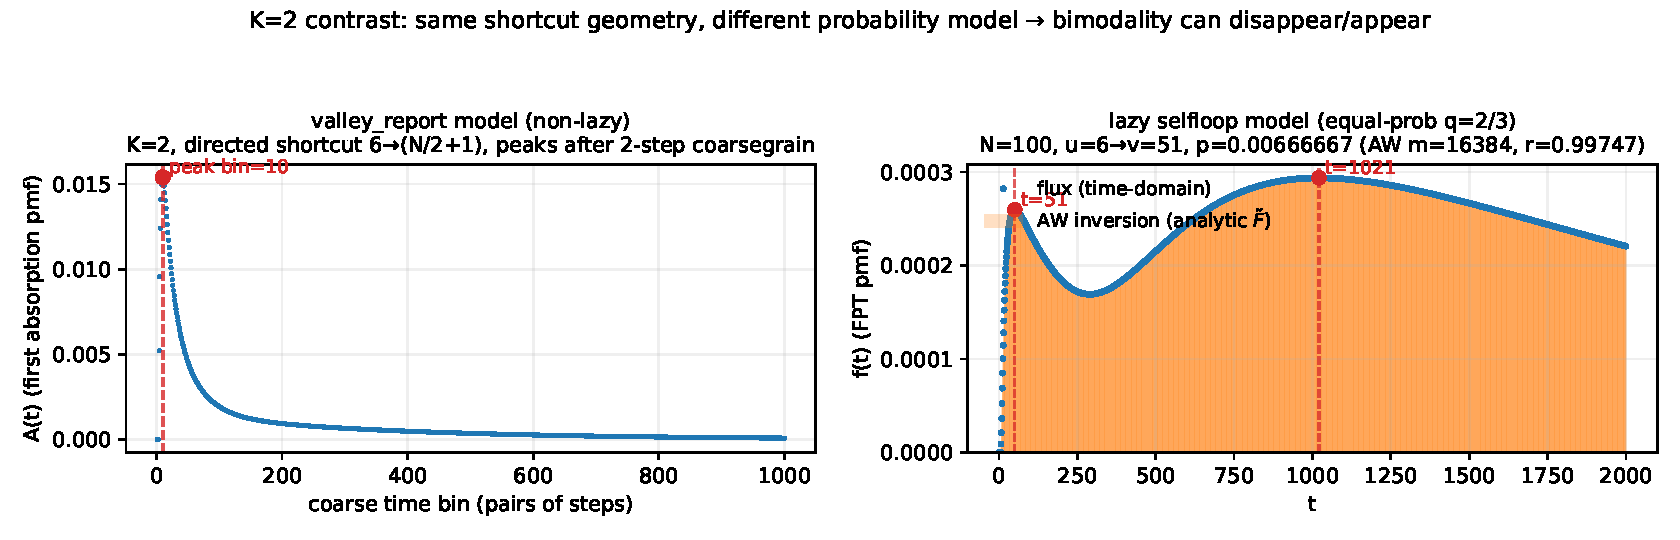
\includegraphics[width=0.96\linewidth]{figures/lazy_ring_flux_bimodality/k2_valley_report_vs_lazy_contrast.pdf}
  \caption{$K=2$ contrast: same shortcut geometry, different probability rule $\Rightarrow$ unimodal vs.\ bimodal behavior.}
  \label{fig:k2-contrast}
\end{figure}

\section{Possible next steps (not executed here)}
To locate the onset of bimodality more systematically, a direct approach is to scan parameter planes and record $(t_1,t_2)$:
\begin{itemize}
  \item \textbf{Scan $(q,p)$ or $(q,\beta)$:} fix a geometry (e.g.\ the paper-like offsets $u=n_0+5$, $v=\mathrm{target}+1$) and scan
  $q\in(0,1)$ with $p\in[0,1-q]$ (or $p=\beta(1-q)$). For each grid point, use AW to produce $f(1..t_{\max})$, compute paper/macro flags and $(t_1,t_2)$, and plot heatmaps (e.g.\ “bimodal vs unimodal” or the late peak time $t_2$).
  \item \textbf{Scan geometry:} for fixed $q,p$, scan endpoints (distance $d$) and relative placements of $(u,v)$; compare “fixed $(u,v)$” vs “allow $(u,v)$ to vary” protocols.
  \item \textbf{Robustness against micro-oscillations:} add a valley-depth or coarse-graining rule (cf.\ the 2-step coarse-grain in \texttt{valley\_report}) and cross-check a few representative points with flux.
\end{itemize}

\section{Reproducibility commands}
\begin{itemize}
\item N=10 overlay (AW vs flux): \path{python3 code/plot_lazy_k2_example.py}
\item N=11 overlay: \path{python3 code/plot_lazy_k2_example.py --N 11 --target 5 --v 5 --tplot 60}
\item heatmap: \path{python3 code/plot_lazy_k2_aw_distance_scan.py --N-min 3 --N-max 60}
\item full scan table: \path{python3 code/scan_lazy_k2_aw_fulltable.py --N-min 3 --N-max 60}
\item multi-panel gallery (even\_small): \path{python3 code/plot_lazy_k2_aw_antipodal_panels.py --group even_small}
\item multi-panel gallery (odd\_small): \path{python3 code/plot_lazy_k2_aw_antipodal_panels.py --group odd_small}
\item multi-panel gallery (even\_medium): \path{python3 code/plot_lazy_k2_aw_antipodal_panels.py --group even_medium}
\item equal4 (paper-like geometry) scan: \path{python3 code/scan_lazy_k2_equal4_paper_geometry.py --N-min 10 --N-max 200}
\item paper-like selfloop vs equal4 comparison: \path{python3 code/plot_lazy_k2_paper_geometry_equal4_compare.py --N 100}
\item small-$p$ bimodal gallery (compact multi-panel): \path{python3 code/plot_lazy_k2_selfloop_smallp_gallery_compact.py --q 0.6666666667 --beta 0.02 --tplot 5000}
\end{itemize}

\appendix
\section{Small-$p$ bimodal gallery (selfloop; paper-like geometry)}
This appendix collects a set of small-$p$ selfloop bimodal curves for the paper-like geometry at $\beta=0.02$ (so $p=0.006666\ldots$),
combined into a compact multi-panel PDF (multiple $N$ cases per page).
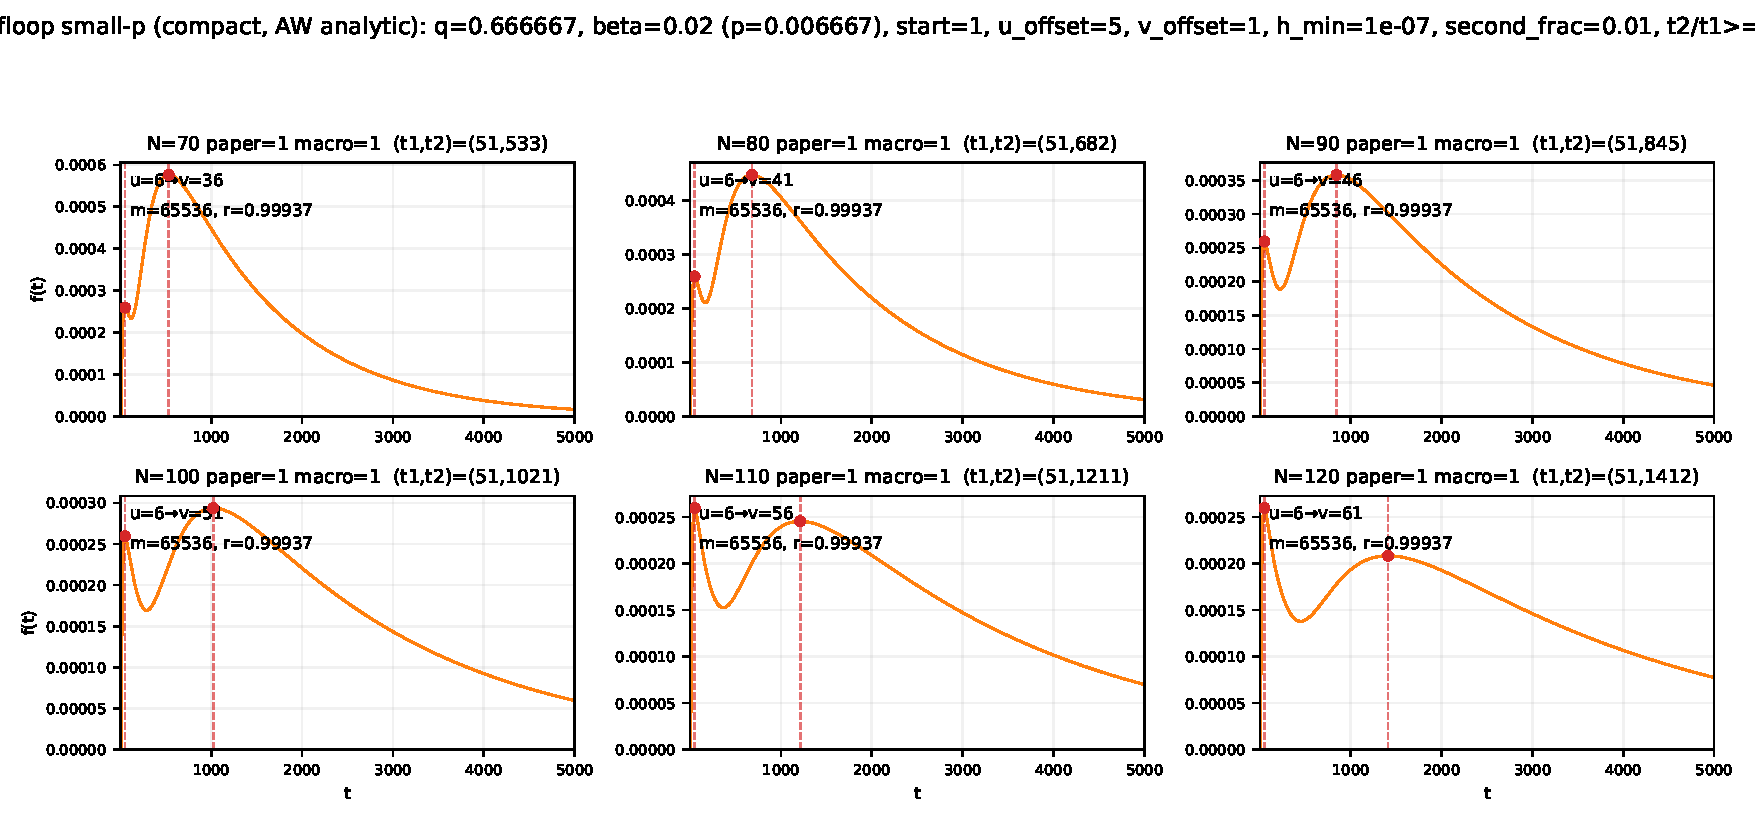
\includepdf[pages=-]{figures/lazy_ring_flux_bimodality/lazy_K2_selfloop_smallp_gallery_compact_beta0.02.pdf}

\section{Supplementary: antipodal AW curves (multi-figure panels)}
For a visual gallery, we also plot AW-inverted pmfs for the (near-)antipodal endpoint $\mathrm{target}=n_0+\lfloor N/2\rfloor$:
\begin{figure}[!htbp]
  \centering
  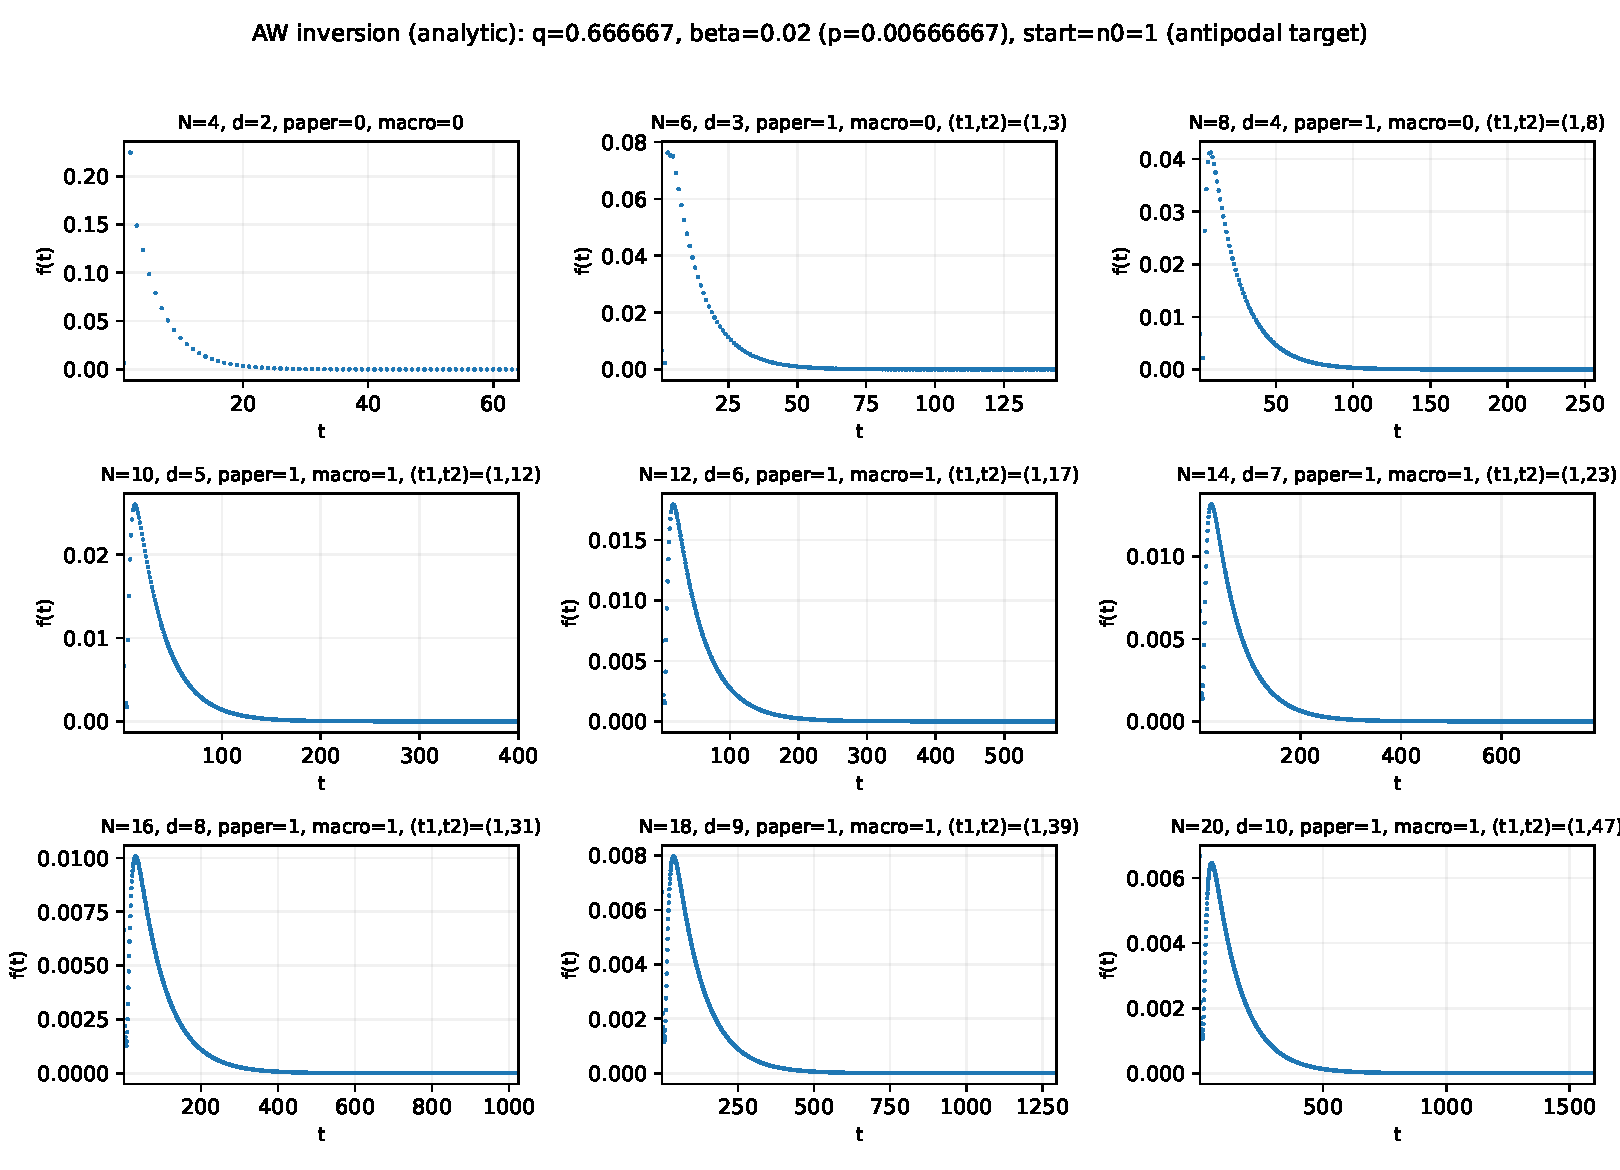
\includegraphics[width=0.92\linewidth]{figures/lazy_ring_flux_bimodality/lazy_K2_aw_antipodal_even_small.pdf}
  \caption{Antipodal examples (even small $N$: $N=4,6,\dots,20$). Titles include paper/macro flags and $(t_1,t_2)$.}
\end{figure}
\begin{figure}[!htbp]
  \centering
  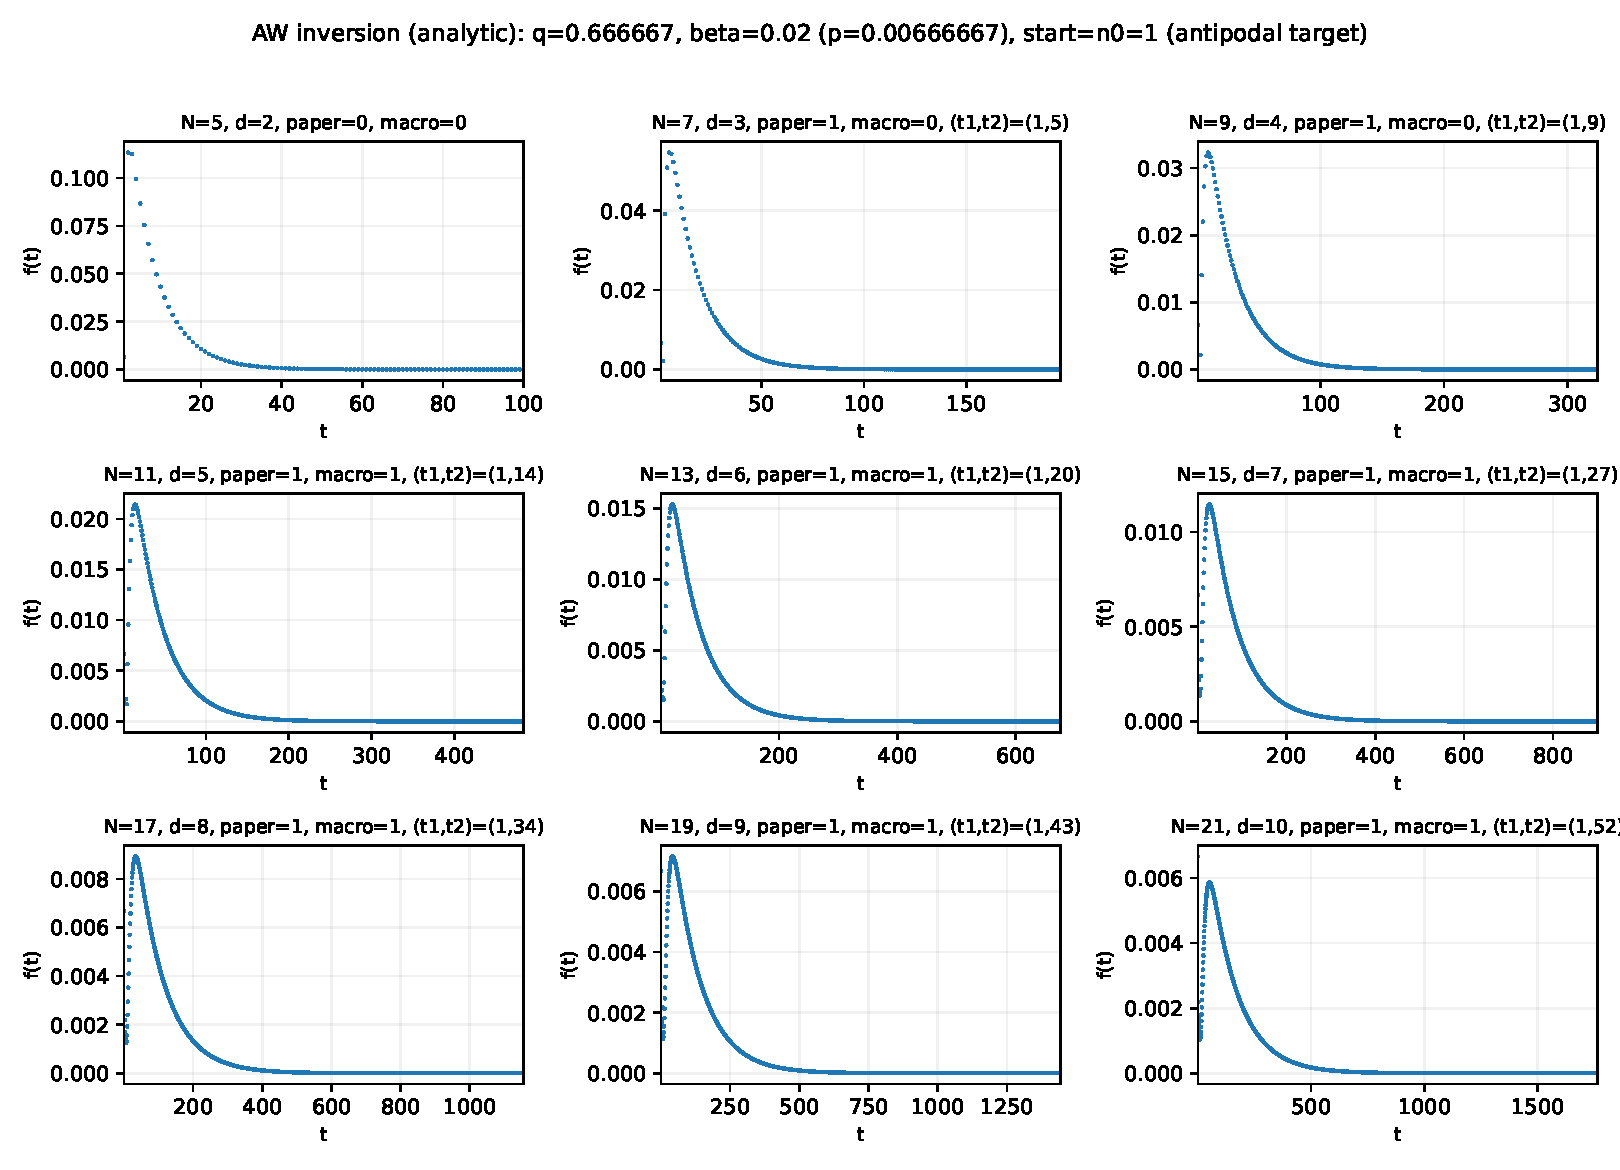
\includegraphics[width=0.92\linewidth]{figures/lazy_ring_flux_bimodality/lazy_K2_aw_antipodal_odd_small.pdf}
  \caption{Antipodal examples (odd small $N$: $N=5,7,\dots,21$).}
\end{figure}
\begin{figure}[!htbp]
  \centering
  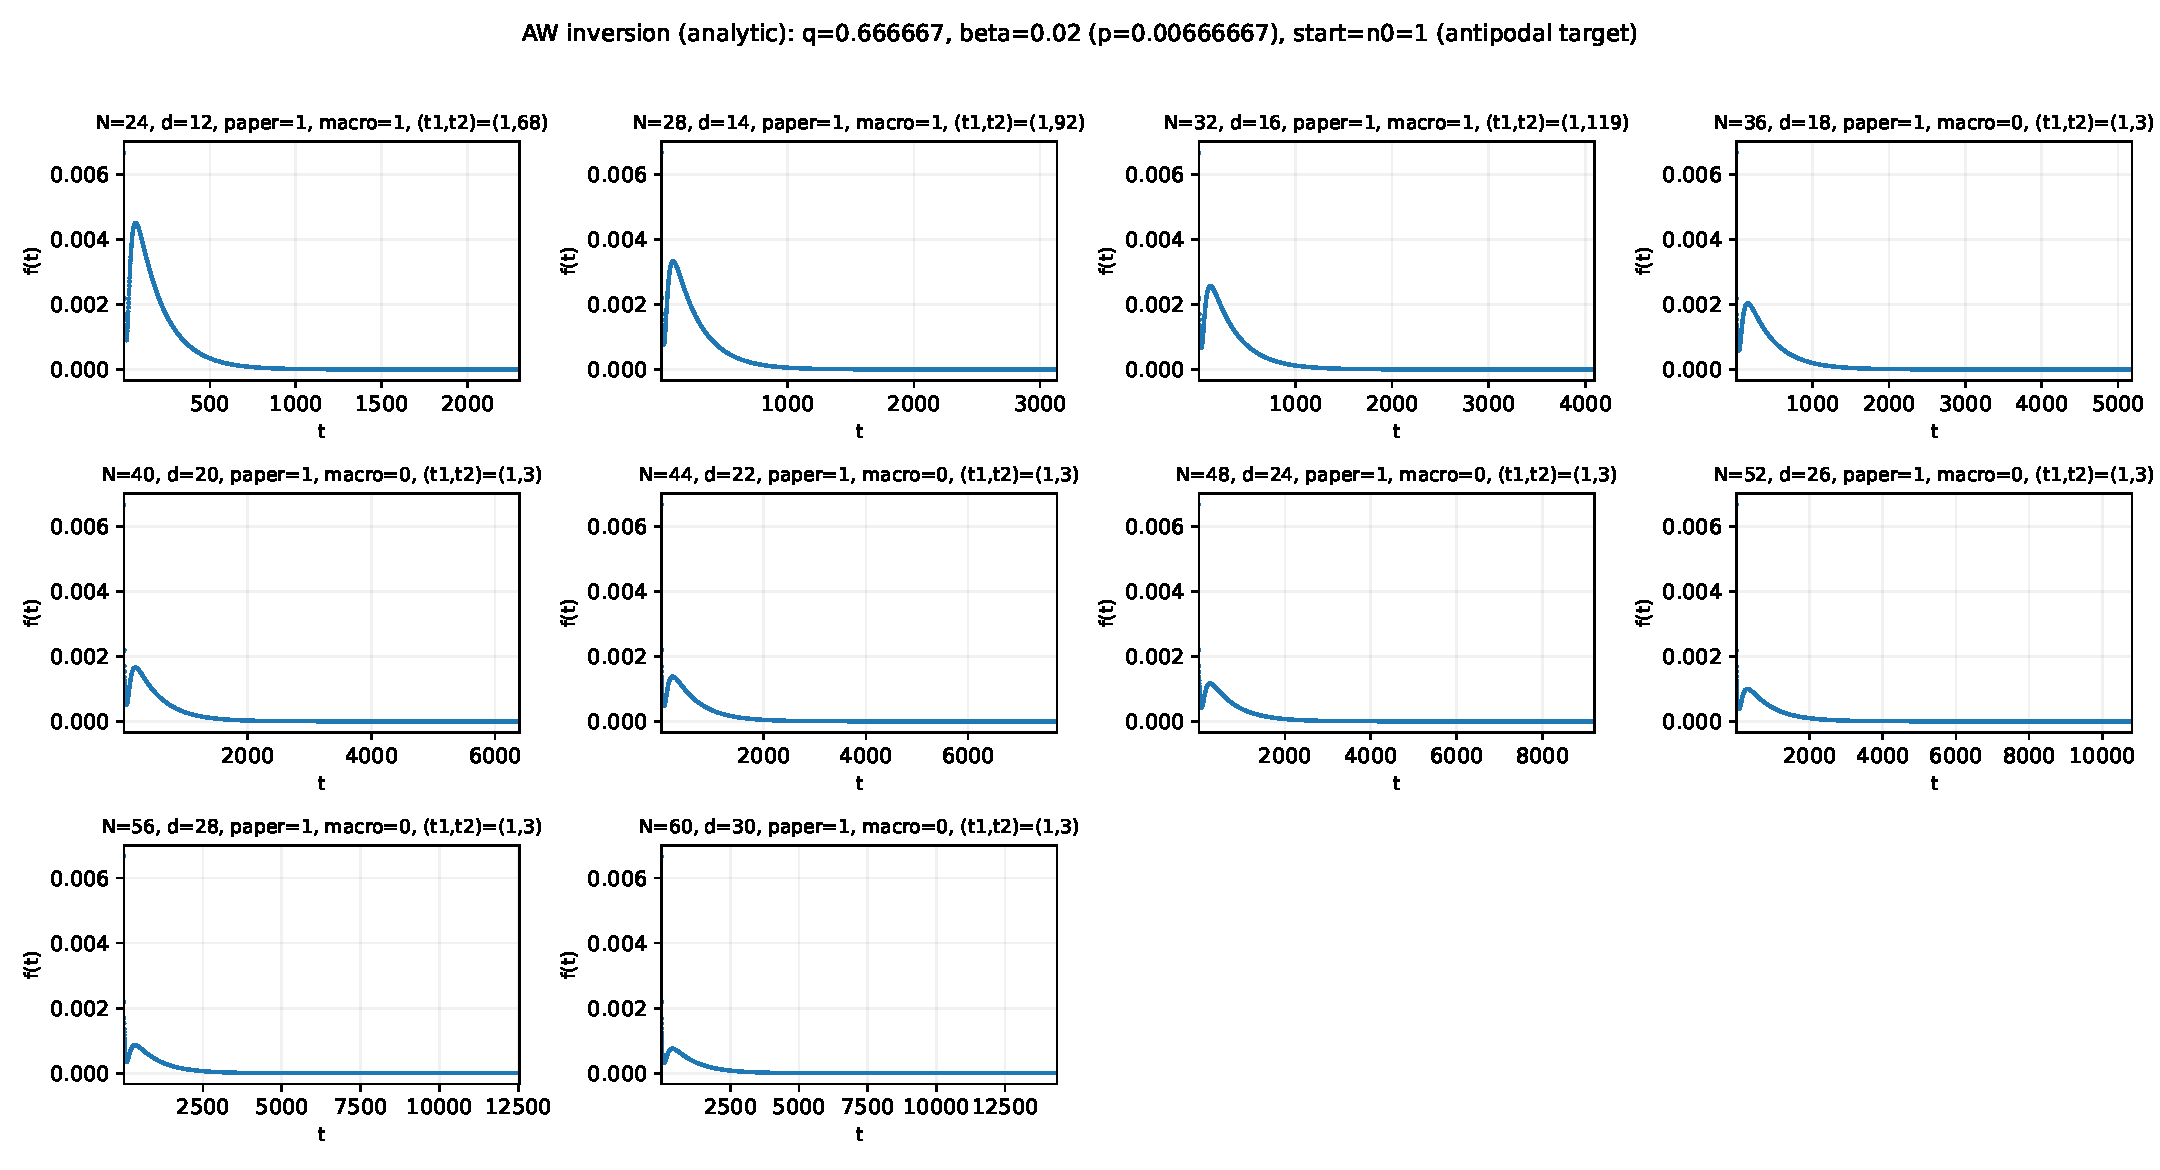
\includegraphics[width=0.92\linewidth]{figures/lazy_ring_flux_bimodality/lazy_K2_aw_antipodal_even_medium.pdf}
  \caption{Antipodal examples (even larger $N$: $N=24,28,\dots,60$).}
\end{figure}

\section{Full scan table}
\scriptsize
\input{tables/lazy_K2_equalprob_full_scan_table_en.tex}

\end{document}
